\documentclass[12pt, a4 paper]{article}
\usepackage{geometry}
\geometry{left=2cm, right=2cm, top=1.5cm, bottom=1.5cm}
\usepackage{amsmath}
\usepackage{amssymb}
\usepackage{amsfonts}
\usepackage{framed}
\usepackage{caption}
\usepackage{indentfirst}
\usepackage{graphicx}
\begin{document}
    %%%%%%%%%%%%%%%%%%%%%%%%%%%%%%%%%%%%%%   Q1   %%%%%%%%%%%%%%%%%%%%%%%%%%%%%%%%%%%%%%%%%
    \begin{framed}
        \section{[Q1]}
        Last class, we mainly talked about unconstrained optimization, especailly the convex set and
         convex function. In convex set part, we talked the definition of convex set and gave some
         concrete examples. Like convex cone, A convex cone is a cone that is convex and a proper 
         cone is a convex cone that does not contain entire lines and has nonempty interior. 
         In convex function part, we talked about the definition and more examples
         of convex function. Besides, operations that preserve convexity were introduced too.
         I learned how to distinguish a strictly convex from convex functions. There will be no 
         linear region in srtictly convex functions.
    \end{framed}

    %%%%%%%%%%%%%%%%%%%%%%%%%%%%%%%%%%%%%%   Q2   %%%%%%%%%%%%%%%%%%%%%%%%%%%%%%%%%%%%%%%%%
    \begin{framed}
        \section{[Q2]}
        done
    \end{framed}

    %%%%%%%%%%%%%%%%%%%%%%%%%%%%%%%%%%%%%%   Q3   %%%%%%%%%%%%%%%%%%%%%%%%%%%%%%%%%%%%%%%%%
    \begin{framed}
    \section{[Q3]}
    Assume we have a concave function $f(\boldsymbol{x}): \mathbb{R}^{N} \to \mathbb{R}$ which is 
concave if for all $\boldsymbol{x}, \boldsymbol{y} \in \mathbb{R}^{N}$, then, it must satisfy,
    $$
        f\left( \theta \boldsymbol{x} + (1-\theta) \boldsymbol{y}
          \right) \geq \theta f(\boldsymbol{x}) + (1-\theta)f(\boldsymbol{y}), 
          \quad \text{for all } 0 \leq \theta \leq 1
    $$

    Now consider $g(\boldsymbol{x}) = -f(\boldsymbol{x})$, according to the definition, we have,
    $$
        -f\left( \theta \boldsymbol{x} + (1-\theta)\boldsymbol{y}  \right) \leq \theta
         \left[-f(\boldsymbol{x})\right] + (1-\theta) \left[-f(\boldsymbol{y})\right],
          \quad \text{for all } 0 \leq \theta \leq 1
    $$
    \indent Apparently, it satisifes the definition of convex function, and $-f(\boldsymbol{x})$
     is convex and vice versa. Hence, we can conclude that,
    $$
    f(\boldsymbol{x}) \text{ is convex} \Longleftrightarrow -f(\boldsymbol{x}) \text{ is convex}
    $$
    \end{framed}

    %%%%%%%%%%%%%%%%%%%%%%%%%%%%%%%%%%%%%%   Q4   %%%%%%%%%%%%%%%%%%%%%%%%%%%%%%%%%%%%%%%%%
    \begin{framed}
    \section{[Q4]}
    \subsection{(a)}
        \begin{align}
        f(\theta \boldsymbol{x} + (1-\theta) \boldsymbol{y}) 
        &= \lVert \theta \boldsymbol{x} + (1-\theta) \boldsymbol{y} \rVert \\
        &\leq \lVert \theta \boldsymbol{x} \rVert + \lVert (1-\theta) \boldsymbol{y} \rVert \\
        &= \left| \theta \right| \lVert \boldsymbol{x} \rVert + \left| (1-\theta) \right| \lvert
        \boldsymbol{y} \rVert \\
        &= \theta \lvert \boldsymbol{x} \rVert + (1-\theta) \lVert \boldsymbol{y} \rVert \\
        &= \theta f(\boldsymbol{x}) + (1 - \theta) f(\boldsymbol{y})
        \end{align}

        Note that $(1)$ to $(2)$ obeys the triangle inequality, and since we have 
    $0 \leq \theta \leq 1$, $(3)$ to $(4)$ holds.
        Hence, $f(\boldsymbol{x}) = \lVert \boldsymbol{x} \rVert$ is convex function.

    \subsection{(b)}
        No norm can be strictly convex.
        The equality holds as long as $ \boldsymbol{x} = k \boldsymbol{y} $, where
         $k$ is a positive constant.
        \begin{align}
            \lVert \theta \boldsymbol{x} + (1-\theta) \boldsymbol{y} \rVert &= 
            \lVert \theta \boldsymbol{x} + (1-\theta) k \boldsymbol{x} \rVert\\
            &= \theta \lVert \boldsymbol{x} \rVert + (1-\theta) k \lVert \boldsymbol{x} \rVert\\
            &= \theta f(\boldsymbol{x}) + (1-\theta) f(\boldsymbol{y})
        \end{align}
    \end{framed}

    %%%%%%%%%%%%%%%%%%%%%%%%%%%%%%%%%%%%%%   Q5   %%%%%%%%%%%%%%%%%%%%%%%%%%%%%%%%%%%%%%%%%
    \begin{framed}
    \section{[Q5]}
    \subsection{(a)}
            Since $f(\boldsymbol{x})$ is convex, then we have,
        $$
        f(\theta \boldsymbol{x} + (1-\theta) \boldsymbol{y}) \leq \theta f(\boldsymbol{x})
         + (1-\theta) f(\boldsymbol{y}), \quad \text{for all } 0 \leq \theta \leq 1
        $$
        \indent Set $g(\boldsymbol{x}) = f(\boldsymbol{x}) - \alpha$, then we can have,
        \begin{align}
            g(\theta \boldsymbol{x} + (1-\theta) \boldsymbol{y} ) &= f(\theta \boldsymbol{x} 
            + (1-\theta) \boldsymbol{y}) -\alpha \\
            &\leq \theta f(\boldsymbol{x}) + (1-\theta) f(\boldsymbol{y}) - \alpha \\
            &= \theta \left[ f(\boldsymbol{x}) - \alpha \right] + (1-\theta) \left[ f(\boldsymbol{y})
             - \alpha \right] \\
            &= \theta g(\boldsymbol{x}) + (1-\theta) g(\boldsymbol{y})
        \end{align}
        
        Note that $(9)$ to $(10)$ is convexity of $f(\boldsymbol{x})$. \\
        \indent If we find 2 points $\boldsymbol{x}, \boldsymbol{y}$ 
        which satisifes $g(\boldsymbol{x}) \leq 0, g(\boldsymbol{y}) \leq 0$, then 
        $$
        g(\theta \boldsymbol{x} + (1-\theta) \boldsymbol{y}) \leq \theta g(\boldsymbol{x})
         + (1-\theta)g(\boldsymbol{y}) \leq 0
        $$
        \indent which means $\theta \boldsymbol{x} + (1-\theta) \boldsymbol{y} \in S_{\alpha}$ \\
        \indent Hence for all $\alpha \in \mathbb{R}$, set $S_{\alpha} = \left\{ 
            \boldsymbol{x}: f(\boldsymbol{x}) \leq \alpha
        \right\}$ is convex.

        \subsection{(b)}
            Set the optimizer as $\boldsymbol{x^{\star}}$ which satisifes $\forall \boldsymbol{x}
             \in dom f, f(\boldsymbol{x^{\star}}) \leq f(x)$
            Define the optimizer set as $S = \left\{ \boldsymbol{x^{\star}} | \forall x
            , f(\boldsymbol{x^{\star}}) \leq f(\boldsymbol{x}) \right\} $.\\
            \indent Let's define 2 points $a, b \in \text{S}$ such that,
            $$
            \forall \boldsymbol{x}, f(\boldsymbol{a}) \leq f(\boldsymbol{x})
             \text{ and } f(\boldsymbol{b}) \leq f(\boldsymbol{x})
            $$ 
            \indent Since $f(\boldsymbol{x})$ is convex, we have the third point $\theta \boldsymbol{a} 
            + (1-\theta) \boldsymbol{b}$ such that,
            $$
            f(\theta \boldsymbol{a} + (1-\theta) \boldsymbol{b}) \leq \theta f(\boldsymbol{a}) + 
            (1-\theta) f(\boldsymbol{b}), \text{ for all } 0 \leq \theta \leq 1
            $$
            \indent Combine the 3 inequalities, we can have,
            \begin{align}
                f(\theta \boldsymbol{a} + (1-\theta) \boldsymbol{b}) &\leq \theta f(\boldsymbol{a}) + 
                (1-\theta) f(\boldsymbol{b}) \\
                &\leq \theta f(\boldsymbol{x}) + (1-\theta) f(\boldsymbol{{x}}) \\
                &= f(\boldsymbol{x})
            \end{align}
            \indent Hence, we can conclude that the third point $\theta \boldsymbol{a} 
            + (1-\theta) \boldsymbol{b} \in \text{set } S.$ and this optimizer set is convex.

        \subsection{(c)}
            In [Q4], we have proved that $f(\boldsymbol{x}) = \lVert \boldsymbol{x} \rVert$ is
             convex. Thus, using the conclusion from [Q5](a), it's obvious that set $\mathcal{B} = \left\{ 
                \boldsymbol{x}: \lvert \boldsymbol{x} \rvert \leq 1
        \right\}$ must be convex. 

        \subsection{(d)}
            It's not convex. There's the counterexample, let $S_{\alpha}$
            $$
            S_{\alpha} = \left\{ 
                x: -e^{x} \leq \alpha
            \right\}
            $$
            \indent There's no doubt $S_{\alpha}$ is convex set, assume $x,y \in S_{\alpha}$, and we have
            $$
            -e^{x} \leq \alpha, \quad
            -e^{y} \leq \alpha
            $$
            \indent And there's the third point $\theta x + (1-\theta) y$ which satisfies,
            \begin{align*}
                -e^{\theta x + (1-\theta) y} &\leq \theta (-e^{x}) + (1-\theta) (-e^{y})\\
                &\leq \theta \alpha + (1-\theta) \alpha \\
                &=\alpha
            \end{align*}
            \indent However, $f(x) = -e^{x}$ is not convex. Hence, the statement if the question
            doesn't hold.
    \end{framed}

    %%%%%%%%%%%%%%%%%%%%%%%%%%%%%%%%%%%%%%   Q6   %%%%%%%%%%%%%%%%%%%%%%%%%%%%%%%%%%%%%%%%%
    \begin{framed}
        \section{[Q6]}
        \subsection{(a)}
        \begin{align}
        f(\theta \boldsymbol{x} + (1-\theta) \boldsymbol{y}) &= \max \left\{f_{1} (\theta \boldsymbol{x} + (1-\theta) \boldsymbol{y}),
          f_2 (\theta \boldsymbol{x} + (1-\theta) \boldsymbol{y}) \right\} \\
         &\leq \max \left\{ \theta f_1(\boldsymbol{x}) + (1-\theta) f_1({\boldsymbol{y}}),
         \theta f_2{\boldsymbol{x}} + (1-\theta) f_2({\boldsymbol{y}}) \right\} \\
         &\leq \theta \max \left\{ f_1(\boldsymbol{x}), f_2(\boldsymbol{x}) \right\} + (1-\theta) \max
         \left\{ f_1(\boldsymbol{y}), f_2(\boldsymbol{y})\right\}
        \end{align}
        \indent where, $(16)$ to $(17)$ is due to $f_1(\boldsymbol{x}) \text{ and } 
        f_2(\boldsymbol{x})$ is convex.\\
        \indent Hence, $f(\boldsymbol{x}) = \max \left\{ f_1(\boldsymbol{x}),
        f_2(\boldsymbol{x}) \right\}$ is convex.


    \subsection{(b)}
    {\centering
    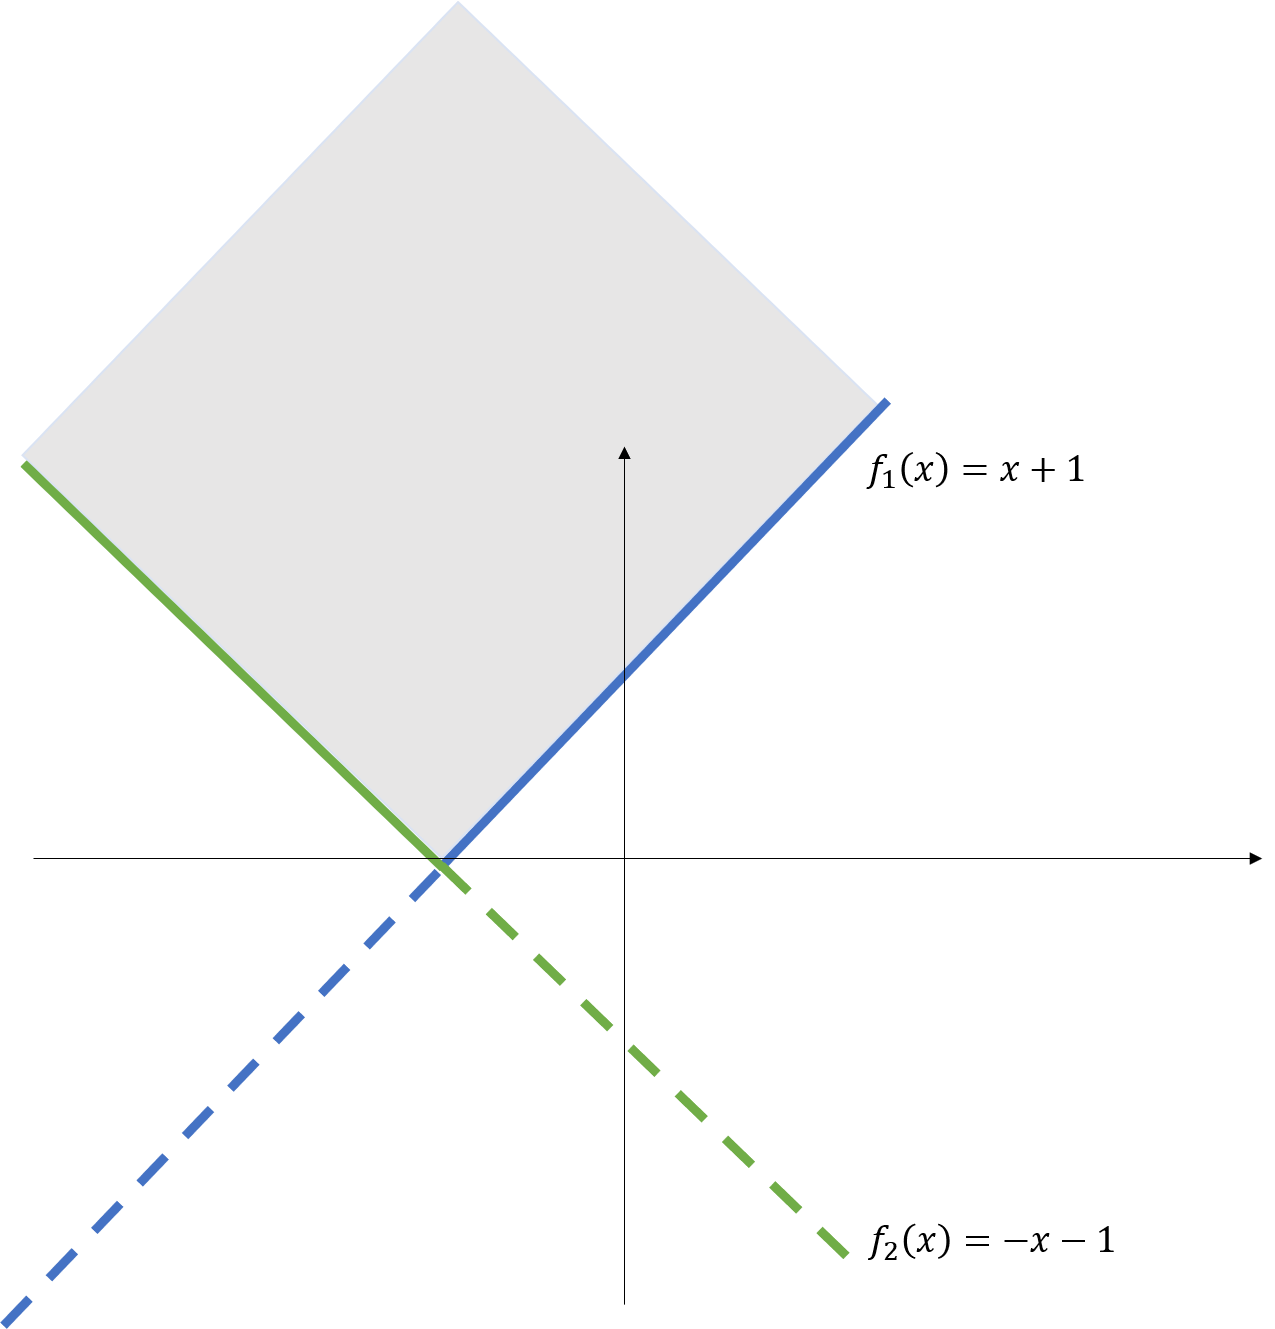
\includegraphics[width=7cm, height=7cm]{1.png}
    \captionof{figure}{Illustration of $f(x) = \max \left\{ f_1(x), f_2(x) \right\}$} 
    }
    In Figure 1, I set $f_1(x) = x+1 \text{ and } f_2(x) = -x-1$, and the shade region is
    $f(x) = \max \left\{ f_1(x), f_2(x) \right\}$. Clearly, the shaded region, namely $f(x)$ 
    is convex.

    
    \subsection{(c)}
    {\centering
    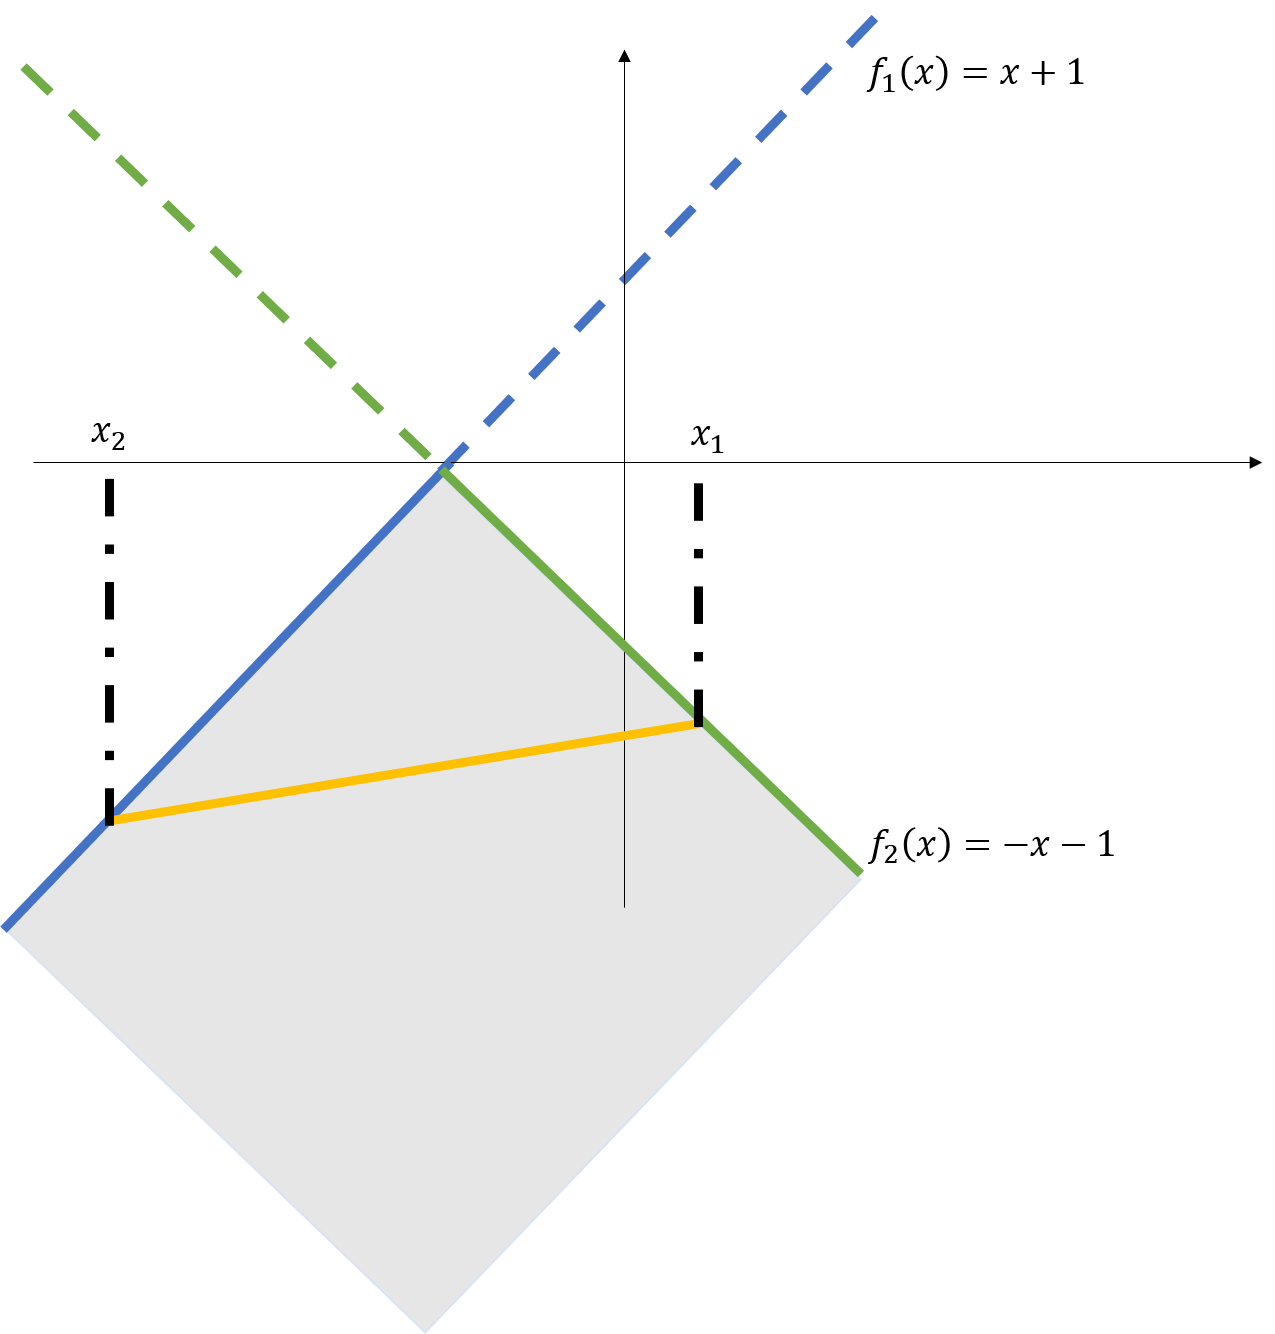
\includegraphics[width=7cm, height=7cm]{2.png}
    \captionof{figure}{Illustration of $f(x) = \min \left\{ f_1(x), f_2(x) \right\}$} 
    }
    Here the yellow line intersected the shaded region with 2 points $x_1, x_2$, where
    $$
    f(\theta x_1 + (1-\theta) x_2) \geq \theta f(x_1) + (1-\theta) f(x_2)
    $$
    \indent Apparently, this is a concave function. It's not a convex function.
    \end{framed}

    %%%%%%%%%%%%%%%%%%%%%%%%%%%%%%%%%%%%%%   Q7   %%%%%%%%%%%%%%%%%%%%%%%%%%%%%%%%%%%%%%%%%
    \begin{framed}
        \section{[Q7]}
        \subsection{(a)}
        According to the Linear Algebra, we know,
        $$
        \lambda_{min}(\boldsymbol{X}) = \min \limits_{\lVert y \rVert = 1} y^T \boldsymbol{X} y 
        $$
        \indent Since $0 \leq \theta \leq 1, y^T\boldsymbol{X_1}y \geq 0 \text{ and } y^T
        \boldsymbol{X_2}y \geq 0$, we can have,
        \begin{align}
            \lambda_{min} \left[ \theta \boldsymbol{X_1} + (1-\theta) \boldsymbol{X_2} \right]
            &=  \min \limits_{\lVert y \rVert = 1} y^T \left[ \theta \boldsymbol{X_1} + (1-\theta) 
            \boldsymbol{X_2} \right] y \\
            &= \min \limits_{\lVert y \rVert = 1} \left[ \theta y^T \boldsymbol{X_1} y + 
            (1-\theta) y^T \boldsymbol{X_2} y \right]\\
            &\geq \theta \min \limits_{\lVert y \rVert = 1} y^T \boldsymbol{X_1} y + (1-\theta)
            \min \limits_{\lVert y \rVert = 1} y^T \boldsymbol{X_2} y \\
            &= \theta \lambda_{min} (\boldsymbol{X_1}) + (1-\theta) \lambda_{min} (\boldsymbol{X_2})
        \end{align}
        \indent where, $(20)$ to $(21)$ is due to $\boldsymbol{\min}$ is a concave function.

        \subsection{(b)}
        Let's denote $\lambda_{max}$ is the largest eigenvalue of of symmetric matrix $X$, then
        we can have,
        $$
        y^{T} \boldsymbol{X} y \leq \lambda_{max} \lVert y \rVert
        $$
        \indent And the set can be described as $\mathbb{S}_{+}^{N} = \left\{ \boldsymbol{X} \lvert
         y^{T} \boldsymbol{X} y \leq \lambda_{max} \lVert y \rVert \right\}$
        Since $f(\boldsymbol{X}) = y^{T} \boldsymbol{X} y$ is an affine function which is convex,
        we can deduce from the conclusion from [Q5](a) that $\mathbb{S}_{+}^{N}$ is a convex set.\\
        \indent The following part proves that $f(\boldsymbol{X}) = y^{T} \boldsymbol{X} y$ is an
        affine function.
        \begin{align*}
        f(\boldsymbol{X}) &= y^{T} \boldsymbol{X} y \\
        &= \sum\limits_{i=1}^{n} \sum\limits_{j=1}^{n} y_{i} x_{ij} y_{j} \\
        \end{align*}
        \indent where, $y_{i}$ indicates the $i$th element of vector $y$ and $x_{ij}$ indicates the $i$th row
        and $j$th coloumn of matrix $\boldsymbol{X}$. \\
        \indent Apparently, it's a linear combination of $x_{ij}$ with its cofficient $\lVert y \rVert$. Hence
        it's an affine function and also a convex function.

        \subsection{(c)}
        I suppose that as long as these convex functions are affine functions like,
        $$
        f_{m}(\boldsymbol{X}) = y_{m}^{T} \boldsymbol{X} y_{m}
        $$
        \indent then it satisfies the requirements. Hence, the set of convex functions must be,
        $$
        S_{f} = \left\{ f_{m}(\boldsymbol{X}) \lvert f_{m}(\boldsymbol{X}) =  y_{m}^{T} 
        \boldsymbol{X} y_{m}) \right\}
        $$
        \indent And $b_{m}$ set is
        $$
        S_{b} = \left\{ 
            b_{m} \lvert b_{m} = \lambda_{\max} \lVert y_{m} \rVert
        \right\}
        $$

    \end{framed}

    %%%%%%%%%%%%%%%%%%%%%%%%%%%%%%%%%%%%%%   Q8   %%%%%%%%%%%%%%%%%%%%%%%%%%%%%%%%%%%%%%%%%
    \begin{framed}
        \section{[Q8]}
        \subsection{(a)}
        $$
        f^{\prime}(x) = 2ax + b
        $$
        $$
        f^{\prime \prime} (x) = 2a  
        $$
        \subsection{(b)}
        $$
        f^{\prime}(x) = \sum\limits_{m=1}^{M} - \frac{a_{m}}{1+e^{a_{m}x}}
        $$
        $$
        f^{\prime \prime}(x) = \sum\limits_{m=1}^{M} \frac{a_{m}^{2}e^{a_{m}x}}{(1+e^{a{m}x})^2}
        $$
    \end{framed}

    %%%%%%%%%%%%%%%%%%%%%%%%%%%%%%%%%%%%%%   Q9   %%%%%%%%%%%%%%%%%%%%%%%%%%%%%%%%%%%%%%%%%
    \begin{framed}
        \section{[Q9]}
        \subsection{(a)}
        $$
        \nabla f(x) = 2\boldsymbol{A} \boldsymbol{x} + \boldsymbol{b}
        $$
        $$
        \nabla^{2} f(x) = 2\boldsymbol{A}
        $$
        \subsection{(b)}
        $$    
        \nabla f(x) = \left[
            \begin{array}{ccc}
                \sum\limits_{m=1}^{M} \frac{-a_{m1}}{1+e^{a_{m}^{T} \boldsymbol{x}}}\\
                \sum\limits_{m=1}^{M} \frac{-a_{m2}}{1+e^{a_{m}^{T} \boldsymbol{x}}}\\
                \vdots\\
                \sum\limits_{m=1}^{M} \frac{-a_{mN}}{1+e^{a_{m}^{T} \boldsymbol{x}}}
              \end{array}
        \right]
        $$
        \indent where, $a_{mi}$ means the $i$th element of column vector $a_{m}$

        $$
        \nabla^{2} f(x) = \left[
              \begin{array}{cccc}
                  \sum\limits_{m=1}^{M} \frac{a_{m1}^{2} e^{a_{m}^{T}\boldsymbol{x}}} {(1+e^{a_{m}^{T} \boldsymbol{x}})^{2}} & 
                  \sum\limits_{m=1}^{M} \frac{a_{m1} a_{m2} e^{a_{m}^{T}\boldsymbol{x}}} {(1+e^{a_{m}^{T} \boldsymbol{x}})^{2}} &
                  \cdots & 
                  \sum\limits_{m=1}^{M} \frac{a_{m1} a_{mN} e^{a_{m}^{T}\boldsymbol{x}}} {(1+e^{a_{m}^{T} \boldsymbol{x}})^{2}}\\
                  \sum\limits_{m=1}^{M} \frac{a_{m2} a_{m1} e^{a_{m}^{T}\boldsymbol{x}}} {(1+e^{a_{m}^{T} \boldsymbol{x}})^{2}} &
                  \sum\limits_{m=1}^{M} \frac{a_{m2}^{2} e^{a_{m}^{T} \boldsymbol{x}}} {(1+e^{a_{m}^{T} \boldsymbol{x}})^{2}} &
                  \cdots &
                  \sum\limits_{m=1}^{M} \frac{a_{m2} a_{mN} e^{a_{m}^{T}\boldsymbol{x}}} {(1+e^{a_{m}^{T} \boldsymbol{x}})^{2}}\\
                  \vdots & \vdots  & \ddots   & \vdots  \\
                  \sum\limits_{m=1}^{M} \frac{a_{mN} a_{m1} e^{a_{m}^{T}\boldsymbol{x}}} {(1+e^{a_{m}^{T} \boldsymbol{x}})^{2}} & 
                  \sum\limits_{m=1}^{M} \frac{a_{mN} a_{m2} e^{a_{m}^{T}\boldsymbol{x}}} {(1+e^{a_{m}^{T} \boldsymbol{x}})^{2}} &
                  \cdots & 
                  \sum\limits_{m=1}^{M} \frac{a_{mN}^{2} e^{a_{m}^{T}\boldsymbol{x}}} {(1+e^{a_{m}^{T} \boldsymbol{x}})^{2}}

              \end{array}
        \right]
        $$
        \indent where, $a_{mi}$ means the $i$th element of column vector $a_{m}$

    \end{framed}

    %%%%%%%%%%%%%%%%%%%%%%%%%%%%%%%%%%%%%%   Q10   %%%%%%%%%%%%%%%%%%%%%%%%%%%%%%%%%%%%%%%%%
    \begin{framed}
        \section{[Q10]}
        \subsection{(a)}
        convex
        \subsection{(b)}
        convex
        \subsection{(c)}
        it's not convex and concave
        \subsection{(d)}
        convex
        \subsection{(e)}
        it's not convex and concave
        \subsection{(f)}
        convex
    \end{framed}

\end{document}